\pagestyle{fancy}
\headheight 20pt
\lhead{Ph.D. Thesis --- N. Leigh }
\rhead{McMaster - Physics \& Astronomy}
\chead{}
\lfoot{}
\cfoot{\thepage}
\rfoot{}
\renewcommand{\headrulewidth}{0.1pt}
\renewcommand{\footrulewidth}{0.1pt}

\chapter{Introduction} \label{chapter1} 
\thispagestyle{fancy} 
%\setlength{\epigraphwidth}{5.5in} \epigraphhead[20]{\epigraph{``To
%    explain all nature is too difficult a task for any one man or even
%    for any one age. 'Tis much better to do a little with certainty,
%    and leave the rest for others that come after you, than to explain
%    all things by conjecture without making sure of any
%    thing.''}
%{%\textit{\\Statement from unpublished notes for the Preface to Opticks (1704)}
%\textsc{\\Sir Isaac Newton} (1643-1727)}}

%Gravity is the glue that holds our Universe together.  It binds the
%gas that forms stars, and is the reason they are rarely found 
%alone. 
%
%One is the lonesliest number.  Thanks to gravity, however, this
%expression rarely applies to stars.  
The vast majority of the stars in our
Universe are found in galaxies, each of which is typically populated
by billions of members.  The hierarchy of stellar communities within
galaxies can be understood if an analogy is made between stars and
people.  In this context, parallels can be drawn between galaxies and
countries, star clusters and cities, as well as multiple star systems
and families.  It is now known that at least half of the stars in
galaxies were born in star clusters \citep[e.g.][]{kroupa02a,
  kroupa02b}, spherical conglomerates 
composed of anywhere from a few hundred to a few million members all
orbiting their common center of mass (see
Figure~\ref{fig:NGC7078}).  Within these stellar 
nurseries, around 50\% of all stars are thought to spend the
majority of their lives in 
close proximity to one or more of their siblings by forming multiple 
star systems \citep[e.g.][]{durisen94, bate97a, bate97b, kroupa01,
  sollima10}.  Most of these are 
binary star systems, which consist of two stars orbiting their common 
centre of mass under the influence of their mutual gravitation
attraction.  Although less common, stable configurations of triple,
quadruple and quintuple star systems also exist, along with even
higher order multiples \citep[e.g.][]{latham05, eggleton08,
  tokovinin08}.  Despite the 
fact that stars typically spend at most a small fraction of their
considerably long lives in even relative isolation, our understanding
of the mechanisms via which the presence of their siblings can affect
their evolution is far from complete.  

\begin{figure} [!h]
  \begin{center}
 \includegraphics[scale=0.5]{Chapter-1/m15_hst.ps}
%    \caption[Plot showing the RA and Dec coordinates for all stars in NGC
%1261]{Right ascension (RA) and declination (Dec) coordinates are shown
%  for all stars in the Milky Way globular cluster NGC 1261.  Using
%  these coordinates, which together form the equitorial coordinate system,
%  an image for the cluster is generated that is projected onto the
%  plane of the sky.
  \caption[An image taken with the \textit{Hubble Space Telescope} of
  the globular cluster NGC 7078]{An image taken with the
    \textit{Hubble Space Telescope} of NGC 7078 (M15), a globular
    cluster in the Milky Way galaxy.  Image credit:  NASA, ESA, and
    The Hubble Heritage Team.
      \label{fig:NGC7078}}
    \end{center}
\end{figure}  

%acts as the catalyst instead of mediates?
Gravity mediates a wide variety of interactions between stars.  Within
the dense cores of star clusters, for instance, strong gravitational 
encounters often occur in which the distance of closest approach is
comparable to the radii of the stars \citep[e.g.][]{spitzer72,
  spitzer75, heggie75, hut83b}.  These encounters often lead to
complex dances that can result in stars being ejected from their host
clusters \citep[e.g.][]{henon69, hut92, kroupa02b, demarchi10}, or even
stellar collisions \citep[e.g.][]{leonard89, sills01}.
Binary stars are also at the
mercy of gravity and, if their orbital separation becomes sufficiently
small, this can lead to the transfer of mass from the surface of one
component to the other \citep{mccrea64}, or even their complete
coalescence \citep[e.g.][]{andronov06}.
Not only are gravitational interactions important for stellar mergers,
they also drive the evolution of star clusters.  Gravity slowly acts
to dissolve clusters, continuously ejecting stars so that they may
join the rest of the Galactic population
\citep[e.g.][]{portegieszwart01}.  It follows that a complete 
understanding of the
dominant physical processes operating in clusters, including how their
stars are formed and the dynamical interactions that cause their stars
to escape, is a key ingredient in piecing together the history of our
Galaxy.  

Mergers are a particularly interesting and important outcome of
stellar interactions.  Observations have revealed 
numerous examples of curious stars and mysterious astrophysical
processes that are thought to be related to stellar mergers
\citep[e.g.][]{sandage53, webbink84, paczynski86, troja10,
  miroshnichenko07, farrell09}.  
%, including
%blue straggler stars (BSs) \citep[e.g.][]{sandage53, sills01,
%  sills02}, Type Ia supernovae \citep[e.g.][]{webbink84}, gamma ray
%bursts \citep[e.g.][]{paczynski86, troja10},
%rapidly rotating B[e] stars \citep[e.g.][]{miroshnichenko07}, and
%intermediate-mass black holes \citep[e.g.][]{farrell09}.  
Many
of these objects are commonly found in dense star clusters, hinting at
the complexity of their dynamical evolution and the potential
importance of dynamics for stellar mergers.  
Although their origins remain unknown, some of these 
objects have served as important tools for furthering our 
understanding of the Universe.  For instance, Type Ia supernovae
have provided the most robust constraints to date for the rate of
Universal expansion \citep[e.g.][]{perlmutter99}.  Despite their 
considerable astrophysical significance, we are far from completely
understanding the physical mechanisms that cause mergers to occur.  

Stellar mergers are but one example of this ubiquitous
physical process, which occurs between objects on many scales.
%The merger of two or more objects is a physical process that occurs
%on many scales.
From colliding galaxies to fusing atoms,
mergers occur on spatial and temporal scales ranging by
many orders of magnitude.  Familiar principles such as conservation of
energy and momentum often apply, however, regardless of scale.  
%appear in every physical subdiscipline.
This is certainly the case for the various forms of dynamical
interactions that lead to mergers.  
% are also ubiquitous
%throughout
%the Universe, occurring on a range of astrophysical scales.  
Examples include chemical reactions in the interstellar medium, strong
gravitational interactions involving massive black holes and even 
encounters between galaxies in galaxy clusters.  
It follows that the development of tools designed to further
our understanding of stellar dynamics and mergers also have
applications for a number of other physical sub-disciplines.
%
%
%This is the case atomic collisions, 
%stellar encounters as well as shock fronts formed from colliding
%molecular clouds.  
%The laws of thermodynamics are also consistently
%relevant regardless of scale.  
%scale.  A good example of this is that gravitationally-bound systems
%can be described as having a negative specific heat \citep{spitzer87}.
%This is a useful concept for understanding stellar evolution and the
%evolution of star clusters.  Similarly, 
%For example, thermodynamic entropy is a useful quantity to consider when
%predicting the structure of the product of a stellar collision
%\citep{lombardi02}.  It is the entropy distributions of the stars
%going into the collision that determine the structure of the collision
%product, with the lowest entropy material settling to the bottom of
%the potential well.
%These examples show that the physics of mergers is a robust subject
%related to a number of physical subdisciplines.

%Gravitational interactions are important for not only stellar mergers,
%but
%also the dynamical evolution of star clusters.  Most stars
%are born in star clusters, but later escape to join the rest of
%the Galactic population.  It follows that a complete understanding of
%the
%dominant physical processes operating in clusters, including how their
%stars are formed and the dynamical interactions that cause their stars
%to escape, is a key ingredient in piecing together the history of our
%Galaxy.  
%Many of these dynamical processes are also ubiquitous
%throughout
%the Universe, occurring on a range of astrophysical scales.  Examples
%include chemical reactions in the interstellar medium, strong
%gravitational interactions at the center of our Galaxy and even
%dynamical interactions between galaxies in galaxy clusters.
%It follows that the development of tools designed to further
%our understanding of stellar dynamics also have applications for a
%number of other physical subdisciplines.

In this thesis, we present statistical and theoretical techniques
related to the physics of mergers.  These are applied to observations
of dense star clusters in order to study the mergers of stars.  In
this chapter, we will outline our motivation for conducting this 
research.  In
Section~\ref{SPs}, we briefly review our current
understanding of stellar evolution theory, and discuss the observed
properties of star clusters and their stellar populations, including
the various types of stellar exotica.  In
Section~\ref{dynamics_intro}, we provide a brief description of the dominant
physical processes that drive the dynamical evolution of star
clusters.  All of these issues are connected in Section~\ref{wheretogo},
where we describe how they have motivated the development of the
techniques that will be presented in this thesis, along with their
application to observations of star clusters.
%In Section~\ref{summary}, we summarize our results and explain how the 
%techniques presented in this thesis are applicable to a wide variety
%of physical processes, ranging from merging galaxies to chemical
%reactions in the ISM.

\section{Stellar Populations in Star Clusters} \label{SPs}

\subsection{Single Star Evolution} \label{standard}

By serving as sites for star formation, star clusters have played a
crucial role in shaping the present-day features of our Galaxy.  And
yet, this is but one example of their 
astrophysical significance.  Star clusters are also ideal
laboratories for learning about stellar evolution.  Historically,
their importance in this regard has stemmed from the often-adopted
assumption that all of the stars in a given cluster were born 
from the same gas cloud at more or less the same time.  If true, star
clusters offer a large sample of stars with a wide range of masses,
but a very narrow range in both age and chemical composition.
Therefore, observations of star clusters offer robust constraints for
stellar evolution theories by providing direct tests for their
predictions for a diverse spectrum of stellar masses of known age and
composition. 

Colour-magnitude diagrams (CMDs) are one of the most
important tools available to astronomers for studying stellar
evolution \citep{hertzsprung09}.  In these diagrams, the
observed surface temperature is 
plotted against luminosity (or brightness) for every star in the 
cluster.  The latter quantity is plotted backwards, and provides a
proxy for colour -- hot stars are blue and cool stars are red.
This creates a characteristic appearance that is observed in all
cluster CMDs.  An example is shown
in Figure~\ref{fig:CMD} for the GC NGC 
6205.  This characteristic shape can be understood by
considering two principles of stellar 
evolution.  The first is called the Vogt-Russell Theorem and states
that the mass, composition and age of a star uniquely determine its radius,
luminosity and internal structure, in addition to its subsequent
evolution \citep{vogt25, russell25}.  The second is simply that the
rate at which a star evolves, and in so doing changes its brightness
and colour, is inversely proportional to some power of its
mass \citep[e.g.][]{iben91}.  It follows that, for a cluster composed
of a large number of stars with a distribution of masses
but similar compositions (at birth) and ages, the most massive stars
are also the most evolved.  Therefore, every evolutionary phase in
the life of a star is typically represented in at least moderately old
clusters, and this causes the distribution of stars in the 
CMD to adhere to the characteristic shape shown in Figure~\ref{fig:CMD}.  
Our understanding of single star evolution is sufficiently
complete that it is now known how this shape changes as a
function of composition and age.  In general, the majority of the features
characteristic of CMDs are well understood, although exceptions
do exist.  Before getting to these in Section~\ref{extra}, we
will review the life cycle of a typical star in our Galaxy and connect
each evolutionary phase to its corresponding location in the CMD.

\begin{figure} [!h]
  \begin{center}
 \includegraphics[scale=0.5]{Chapter-1/thesis_fig2.ps}
    \caption[CMD for the Milky Way globular cluster NGC
    6205]{Colour-magnitude diagram for the Milky Way globular cluster 
      NGC 6205.  The data used to create this plot were taken from
      \citet{sarajedini07}.  %The units on the x- and y-axes correspond
%      to photometric magnitudes in the F606W and F814W bands, which
%      are used to estimate stellar brightnesses and colours.  The
%      x-axis plots the quantity F606W-F814W, whereas the y-axis plots F814W.
%      Absolute magnitudes are shown, converted from apparent
%      magnitudes using the
%      distance modulii and extinctions provided in \citet{dotter10}.  
      As described in the text, the x-axis can be read as temperature
      (or, equivalently, colour), 
      which increases from right to left (red to blue).  On the
      y-axis, brightness increases from bottom to top.  
      Labels for blue straggler (BS), red giant branch (RGB), horizontal
      branch (HB), extended horizontal branch (EHB), asymptotic giant
      branch (AGB), Hertzsprung gap (HG), main-sequence turn-off (MSTO) and
      main-sequence (MS) stars are shown.  Stars with large photometric errors
      have been omitted from this plot. 
      \label{fig:CMD}}
    \end{center}
\end{figure}

Most of the star clusters in our Galaxy were born from gas clouds
composed primarily of hydrogen and, to a lesser extent, helium (as
well as heavier elements in trace amounts) \citep[e.g.][]{lada85, pringle89}.  
Gravity contracted the gas into clumps, which grew increasingly
hot and dense as they accreted material from the surrounding medium.
When the central temperature of a clump becomes sufficiently high (on
the order of $10^7$ K), hydrogen is ignited at its centre.  A star is
born.  This marks 
the beginning of the main-sequence (MS) phase, during which
time hydrogen is fused into helium in the stellar core.

Let us consider the life of a typical low-mass star in the Milky Way, from
beginning to end.  Most of the stars in our Galaxy have low
masses roughly spanning the range $0.08 \lesssim$ m $\lesssim 2.0$
M$_{\odot}$ \citep[e.g.][]{kroupa02a}.  There are two reasons for this.
First, the
least massive stars are also the longest lived.  Second, 
\citet{salpeter55} showed that the initial distribution of
stellar masses for stars in the solar-neighbourhood with masses in the
range $0.4 - 10$ M$_{\odot}$ can be described
by a power-law form with an index $\alpha \sim 2.35$.  Today, we know
that the distribution flattens below $\sim 0.5$ M$_{\odot}$, however
the primary conclusion is the same:  most of the stars in our Galaxy
have masses lower than that of our Sun.  What's more, most of these
are MS stars since, for stars of very low-mass, the time-scale for this
evolutionary phase exceeds the age of the Universe.  
%The outcome of
%the complex interplay of physical processes competing 
%within stars to drive their evolution depends somewhat sensitively on
%their mass.  As a 
%result, stellar evolution varies considerably between low- and
%high-mass stars.  Below, we focus our description of this evolution to
%stars with masses $\lesssim 2.0$ M$_{\odot}$.

Nuclear reactions in the stellar core release heat, and are the
primary source of energy generation within stars, driving their high
luminosities \citep[e.g.][]{clayton68}.  The transport of energy
outward within stars in turn 
causes their compositional and structural profiles to evolve.  This
occurs on a typically slow time-scale on the order of millions of
years or longer \citep[e.g.][]{kippenhahn90, maeder09}.  Both the rate
and outcome of the complex interplay of physical processes occurring
within stars to drive their evolution depend somewhat sensitively on
their mass.  As a 
result, stellar evolution varies considerably between low- and
high-mass stars.  Below, we focus our description of this evolution to
stars with masses $\lesssim 2.0$ M$_{\odot}$.

The MS crosses the CMD from bottom right to top left, as shown in
Figure~\ref{fig:CMD}.  During the MS phase, the radius (and hence 
surface temperature) and luminosity
of a star are primarily determined by its mass, however its age and
initial composition also contribute \citep[e.g.][]{iben91, tout96}.  As a
result, the lowest mass stars in a cluster occupy 
the bottom right end of the MS, with stellar mass increasing 
upward and blue-ward.  Most stars spend the majority of
their lives on the MS slowly converting hydrogen into helium in their
cores.  After slowly increasing their
radius and luminosity by a factor of about 2.5-3, stars reach the end
of the MS phase of their evolution \citep{eggleton06}.  This can
roughly be defined as the point at which the hydrogen fuel within a
central core containing about 10\% of the star's mass has run out.  
Found at the left-most tip of the MS in the CMD, called the
main-sequence turn-off (MSTO), the most massive MS 
stars are in the process of depleting their hydrogen fuel in and near
their centres.  At this point, loosely
referred to as the terminal-age main-sequence (TAMS), stars leave the
MS and start moving to the right across
the CMD, becoming increasingly red.  

The stellar evolution time-scales shorten considerably at this point, and
the helium core begins to contract while the envelope expands.  This
causes a drop in the surface temperature of the star, causing it to
move horizontally across the CMD, crossing what
is called the Hertzsprung gap (Figure~\ref{fig:CMD})
\citep[e.g.][]{popper80}.  The reason for 
this rapid reddening can be understood as follows.  Once the
surface temperature drops well below about $10^4$ K, the primary
mechanism of energy transport in the envelope changes
\citep{eggleton06}.  This is
because the drop in temperature
allows free electrons to recombine with free protons to form
hydrogen atoms, which 
can then act to absorb out-going radiation.  This presents a challenge
for the star since energy still needs to be
transported outward from its nuclear-burning centre, yet radiation can
no longer leak out freely.  To compensate,
convection takes over as the dominant form of energy transport
\citep[e.g.][]{bohm-vitense58}.  As
the convective 
base of the envelope deepens, stars of a given luminosity and mass
converge to an approximately unique radius.  The change in stellar
radius that occurs during this short-lived phase of evolution can
range from a factor of less than two for very low-mass stars to a
factor of $\gtrsim 100$ for very massive stars \citep{iben91}.  This
marks the beginning 
of the red giant branch (RGB) phase of evolution, and the base of its
corresponding sequence in the CMD (Figure~\ref{fig:CMD}).  

Due to the unique envelope structure created by the deepening of the
convective envelope, stars of a given mass but different luminosities
must lie on a roughly vertical locus in the CMD
\citep{hayashi62}.  This structure also 
causes the stellar luminosity to increase steeply as a function of the
mass of the helium core \citep[e.g.][]{iben68}.  As hydrogen burning
progresses in 
a shell immediately outside the core, the helium that is produced
rains down onto it, slowly increasing its mass.  This in turn causes
the star to brighten by up to several orders of 
magnitude and, in so doing, ascend the RGB in the CMD.  

Eventually, the mass and temperature of the helium core reach $\sim
0.47$ M$_{\odot}$ and $\sim 10^8$ K, respectively, although the
precise values depend on both the total stellar mass and chemical
composition \citep{eggleton06}.  It is at this 
point that helium ignites, producing mainly carbon at first, although
later the production of oxygen takes over.  The horizontal branch (HB) in
CMDs (Figure~\ref{fig:CMD}) corresponds to
the core-helium burning phase.  It is not clear why HBs show such a
large spread in their colours since, in principle, both the luminosity
and surface temperature should be roughly constant for core
helium-burning stars.  This mysterious and ubiquitous feature of CMDs
marks a significant gap in our understanding of stellar evolution
theory.  We will return to the curious HB morphologies observed in
the CMDs of old star clusters in Section~\ref{HBs_intro}.

Within about $10^8$ years of the onset of core helium-burning,
low-mass stars will typically possess a core composed of carbon and
oxygen with a mass of $\sim 0.55$ M$_{\odot}$ \citep{iben74}.  The
core is surrounded by a much less massive shell composed primarily of
helium and next to no hydrogen.  This, in turn, is surrounded by an
envelope of unprocessed material extending out to 30-50 R$_{\odot}$
from the core \citep{maeder09}.  Two burning shells now power the
star as it continues 
its rise in luminosity above the RGB.  The sequence in the CMD
corresponding to this phase of evolution is called the asymptotic
giant branch (AGB).  As this phase progresses, the radius and
luminosity of the star
continue to grow and severe mass-loss typically occurs due to
powerful stellar winds.

The life of a typical low-mass star ends when the last of its
envelope is burnt, leaving its luminosity to plummet by several
orders of magnitude and its surface temperature to increase
dramatically.  The product is an incredibly dense remnant composed
of carbon and oxygen called a C/O white dwarf (WD) \citep{iben74}.  
% ALISON THINKS THE BELOW SHOULD BE 8 INSTEAD OF 2.  CHECK!!!
This the case for stars with masses up to $\sim 2$ M$_{\odot}$ when
mass-loss on the AGB is factored in \citep{eggleton06}.  For stars
more massive than 
this, stellar death can be considerably more dramatic, ending in the
ignition of carbon and a subsequent thermonuclear explosion.  As
previously explained, these stars are short-lived and do not occur
commonly in old star clusters, which will be the focus of this
thesis.  Therefore, we refer the interested reader to
\citet{clayton68} and \citet{maeder09} for descriptions of the
evolution of massive stars.

\subsection{Additional Features of Colour-Magnitude Diagrams} \label{extra}

There remain several features characteristic of CMDs that cannot be
explained by standard single star evolution.  In order to
account for their existence, it is 
necessary to invoke the aid of other physical processes known to be
operating in star clusters, such as 
binary star evolution and stellar dynamics.  As described in the
subsequent sections, these processes are thought to be responsible for
producing various types of exotic stellar populations and multiple
star systems.  These curious objects typically appear as outliers in
CMDs, and do not fall on any single star evolution tracks.  
%\subsubsection{Mysterious Features of CMDs and Stellar
%Exotica} \label{exotica}
We will discuss the various mysterious features of CMDs and types of
stellar exotica known to populate star
clusters, and review the currently favoured hypotheses for their
origins.

\subsubsection{Horizontal Branch Morphology} \label{HBs_intro}

The horizontal branches of star clusters in the Milky Way have been
observed to display a range of morphologies.  That is, most CMDs have
a horizontal sequence that extends blue-ward from the top of the red
giant branch, and this is referred to as the horizontal branch.
However, the length and appearance of this sequence varies
considerably from cluster-to-cluster and, in some cases, it makes a
sharp vertical transition to dimmer luminosities at its blue-most 
tip.  %The vertical portion of the sequence is often called the
%extended horizontal branch (EHB).  The appearance of the HB in the CMD
CMDs are shown in Figure~\ref{fig:HB_CMDs} for four
different clusters, each of which has a distinct HB morphology.  The
source of this 
variance is unknown, however our current best guess is mass-loss due
to stellar winds, most likely on the RGB \citep[e.g.][]{iben74, dotter10}.
The more mass-loss that occurs, the 
smaller the mass of the remaining envelope.  The surface temperature
increases with decreasing envelope mass since this leaves more of the
hot core exposed.  Consequently, the amount of mass-loss is thought to
determine the colours of HB stars, with stars that experience the
greatest loss in mass ending up the bluest.  In order to reproduce the
observed surface temperatures of the hottest HB stars, the envelope
must lose a mass of 0.2-0.3 M$_{\odot}$ \citep{eggleton06}.  This
seems reasonable and agrees rather well with empirical estimates
\citep[e.g.][]{judge91}.  It is
not yet clear, however, why stars of comparable mass in the same
cluster would experience such different degrees of mass-loss.  It is
also unknown how or why this mass-loss distribution should change from
cluster-to-cluster, although the rate of mass-loss is thought to 
depend on metallicity \citep[e.g.][]{reimers75}.

\begin{figure} [!h]
  \begin{center}
 \includegraphics[scale=0.5]{Chapter-1/thesis_fig3.ps}
    \caption[CMD sections for the Milky Way globular clusters NGC
    6205, NGC 104, NGC 1261 and NGC 6934]{Colour-magnitude diagram sections
      for the Milky Way globular clusters NGC 104 (top left inset),
      NGC 6205 (top right inset), NGC 1261 (lower left inset) and NGC 6934
      (lower right inset).  Note the distinct HB morphology 
      characteristic of each cluster.  Blue stragglers are also
      clearly visible just brighter and bluer than the MSTO.  The data
      used to create this plot were taken from 
      \citet{sarajedini07}.  %The units on the x- and y-axes correspond
%      to photometric magnitudes in the F606W and F814W bands.  As
%      before, the x-axes plot F606W-F814W, whereas the y-axes plot
%      F814W.  Once again, absolute magnitudes are shown, 
%      converted from apparent magnitudes using the
%      distance modulii and extinctions provided in \citet{dotter10}.
      \label{fig:HB_CMDs}}
    \end{center}
\end{figure}

Previous studies have confirmed that the 
observed differences in the HBs of Milky Way clusters
are related to metallicity \citep{sandage60}.  This does not tell the
whole story, however, since at least one
additional parameter is required to explain the spread in their
colours (see Figure~\ref{fig:HB_CMDs}).  Many cluster properties have been
suggested as possible 
Second and Third Parameters.  These include age, the 
cluster luminosity and central density.  Unfortunately, no 
definitive candidates have as of yet been 
identified \citep[e.g.][]{rood73, fusi93}.  Notwithstanding,
observations have revealed several peculiar trends for this curious
stellar population in individual clusters.  For instance,
\citet{saviane98}
presented evidence that blue HB stars could be more centrally
concentrated than red HB stars in the cluster NGC
1851.  Conversely, \citet{cohen97} showed that blue HB stars could be
centrally depleted relative to other stellar types in the cluster NGC
6205.  To date, no clear evidence has been found linking the spatial 
distributions of HB stars to any global cluster properties.

The bluest HB stars are often called extreme horizontal branch (EHB)
stars.  It has been
suggested that RGB stars can shed their entire envelopes and still
ignite helium as EHB stars \citep{dcruz96}.  Moreover, it is thought
that EHB stars could skip the AGB phase and evolve into WDs directly
\citep[e.g.][]{maeder09}.  
EHB stars also go by the name of sub-dwarf B (sdB) stars.  Both 
are core-helium burning stars with very small outer envelopes.  
%,
%however they are typically found in the field of our Galaxy rather than
%in clusters (although we note that the distinction that EHB stars
%are only found in clusters and sdB stars are only found in the field
%is not always strictly adhered to throughout the literature).  Apart
%from their preferred location in our Galaxy, the distinction between
%EHB and sdB stars is unclear.  
%The only exception to this is that
Interestingly, EHB stars in the field tend to have binary companions
\citep{maxted01}.  This could be interpreted as evidence that the 
presence of a binary companion is responsible for causing the dramatic
loss of envelope mass.  On the other hand, most
EHB stars in clusters have been shown to lack a binary companion
\citep[e.g.][]{monibidin06, monibidin09, monibidin11}.  Consequently,
the mechanism responsible for (at least) \textit{their} extreme mass-loss is
still less clear. 

%Try to work in a few short sentences of two or three words for
%oomph/flare.  e.g. At this point, the star gets bright.  Incredibly bright. 
%More analogies/metaphors?

\subsubsection{Blue Stragglers} \label{BSs}

First discovered by \citet{sandage53}, blue straggler stars occupy the
region of the CMD that is just brighter and bluer than the MSTO (see
Figure~\ref{fig:HB_CMDs}).  That
is, they appear as an extension of the main-sequence.  And yet, if all
of the stars in a cluster were born at more or less the same time,
then standard single star evolution predicts that this region
of the CMD should be bare.  Normal MS stars that are of sufficiently
high mass to occupy this region should have long ago evolved onto the
RGB and beyond.  The presence of BSs in star clusters therefore
defies the predictions of single star evolution theory, and signifies 
another one of its mysteries.
%One important example of the interplay that occurs in star clusters
%between stellar evolution and stellar dynamics can be found in the
%study of blue straggler stars.  

This puzzle can perhaps be solved if blue stragglers are produced 
via the addition of fresh hydrogen to the cores of normal 
main-sequence stars \citep[e.g.][]{sills01}.  This is the
currently favoured origin for BSs.  It can occur
via multiple channels, most of which involve the mergers of low-mass
MS stars.  Stars in binaries can be driven to merge if enough orbital
angular momentum is lost.  This can be
mediated by dynamical interactions with other stars
\citep[e.g.][]{leonard89, leonard92}, magnetized
stellar winds \citep[e.g.][]{ivanova03}, tidal dissipation
\citep[e.g.][]{cleary90, chen08b} or even an outer triple companion
\citep[e.g.][]{fabrycky07, perets09}.  Alternatively, stars
can collide directly, although this is also thought to usually be
mediated by multiple star systems \citep{leonard89}.  Stars in close
binaries
can transfer mass if their orbital separations become sufficiently
small for one of the components to over-fill its Roche lobe.  This 
can also deliver fresh hydrogen to normal MS stars and in so doing
produce BSs.  

Whatever the
dominant BS formation mechanism(s) operating in dense star clusters,
dynamical interactions are sufficiently common that they should play
at least some role.  For example,
even if blue stragglers are formed as a result of binary evolution
processes such as mass-transfer, the progenitor binaries themselves
are expected to have experienced at least one dynamical interaction
over the course of their lifetime \citep[e.g.][]{hut83b, leonard89,
  davies04}.  
It follows that the study of BSs in star clusters offers an indirect 
means of probing the interplay between stellar evolution and stellar
dynamics. 

In order to explain recent observations of BS populations in star
clusters, it has been suggested that several BS formation mechanisms
operate simultaneously.  For example,
several studies have reported a bi-modal radial distribution for blue
stragglers \citep[e.g.][]{ferraro97, ferraro99, ferraro04, lanzoni07,
  geller08}.  That is, the number of BSs is the highest in the central
cluster regions, then falls off as the distance from the cluster
centre increases but eventually rises
again in the cluster outskirts.  This has primarily been observed in
globular clusters (GCs), which are particularly massive, dense and old star
clusters 
usually found in the outer reaches of our Galaxy.  One theory proposed
to explain this
result is that the blue stragglers found in the cluster core were
formed from collisions, whereas
those in the cluster outskirts were formed from binary mass-transfer
\citep{ferraro04}.  This hypothesis is motivated by the fact that the
time-scale for collisions to occur between stars is very short in the
core, but drops off considerably in the cluster outskirts where the
stellar densities are much lower \citep{leonard89}.  Alternatively, it
has been suggested that the blue stragglers in the cluster
outskirts could have been formed in the core but were later kicked out
as a result of dynamical encounters involving binary stars
\citep[e.g.][]{sigurdsson93, mapelli06}.

%Using the techniques presented in this thesis, \citet{knigge09}
%showed that blue stragglers have a binary origin in 
%even the dense cores of globular clusters.  This came as something of
%a surprise since theoretical estimates suggest that the rate of
%collisions between single stars should be very high in the cores of
%GCs.  Shortly after this discovery, a spectroscopc survey of the old
%open cluster NGC 188 performed by \citet{mathieu09} revealed that
%most, if not all, of its BSs have binary companions.  Open clusters
%are characterized as having masses, 
%densities and ages that are lower than their globular counterparts by
%up to several orders of magnitude.  In most cases, this means that
%close dynamical interactions between stars, including collisions, do
%not occur very often.  NGC 188 is a special case, however, since it
%has a mass, density and age closer to what is 
%typically observed for globular clusters.  

A spectroscopic survey of the cluster NGC 188 performed by
\citet{mathieu09} revealed that most, if not all, of its BSs have
binary companions.  \citet{mathieu09} proposed that their results are
consistent with the general picture that both mass-transfer 
and mergers are simultaneously producing BSs in NGC 188, which is also
consistent with the results of \citet{chen08a}.  The latter authors fit
theoretical stellar evolution tracks to the observed colour-magnitude
diagram for NGC 188.  Based on their results, they argue that most BSs
in this cluster are too massive to have formed from mass-transfer
alone.  If true, this suggests that many BSs in NGC 188 must be the
products of stellar mergers.  In support of this, \citet{perets09}
argued that the results of \citet{mathieu09} can be
explained if triple stars play an important 
role in BS formation by acting as catalysts for mergers
\citep{perets09}.  Triple stars
can evolve internally by transferring angular momentum between their
inner and outer orbits.  This can cause the eccentricity of the inner
binary to increase dramatically \citep{kozai62}.  Tidal 
friction can then act to reduce the orbital separation by removing
orbital energy from the inner binary at each periastron passage
\citep{fabrycky07} (the term periastron refers to the point of closest
approach for an eccentric binary orbit).

Blue stragglers have also been found in the field of our Galaxy.
Observations of these BSs suggest that both mass-transfer and binary
coalescence are occurring.  For example,
\citet{distefano10} recently reported the discovery of two BSs with
white dwarf companions in the field of our Galaxy.  The authors
suggest that these BSs were
formed from mass-transfer when the white dwarf progenitors
evolved to ascend the RGB and in so doing over-filled their
Roche lobes.  Moreover, \citet{brown10} discovered a $\sim 9.1$
M$_{\odot}$ hypervelocity MS star in the field.  The
authors argue that it must be a blue straggler since its flight time
from the Milky Way (MW) exceeds its MS lifetime.  They conclude that
this BS must 
be the product of a close binary that coalesced sometime after being
ejected from the Galactic centre.  This could explain its
hypervelocity provided its ejection was caused by a dynamical
interaction involving the central massive black hole.

Several spectroscopic studies have also been performed to study individual
BSs in clusters.  For example, at
least two BSs in the globular cluster 47 Tuc have been found with masses
exceeding twice that of the main-sequence turn-off (MSTO)
\citep{shara97, knigge08}.  The large masses of these BSs suggest that
they are the products of the mergers of two or more low-mass MS stars.
Another similarly massive BS was reported by \citet{vandenberg01} in
the old open cluster M67.  This BS is thought to be a member of a
triple star system that contains not one, but two BSs
\citep{sandquist03}.  BSs have been identified in both binaries and
triples in several other clusters as well, including the open cluster
NGC 6819 \citep{talamantes10}.

\subsubsection{Binary Stars}

Unresolved binary stars pollute the CMDs of star clusters, which 
become peppered with peculiar outliers that do not fall on any single 
star evolution tracks.  This is because clusters are located at
sufficiently great distances from us that the components of a given 
binary pair are indistinguishable and they appear as a single object.  
The combined light of the binary components blends together, producing a 
combination of colour and brightness that ordinary single stars are
never expected to display over the course of their
evolution.  This typically creates a secondary sequence in cluster CMDs
located above the MS \citep[e.g.][]{milone08}.  The reason for this is that
most cluster binaries are composed of normal MS stars 
\citep[e.g.][]{geller08}, and the combined 
light of their components makes these binaries appear slightly
brighter than ordinary single MS stars.

There are many examples of objects that are almost certainly bonafide
cluster members but appear in curious locations in the CMD.  Examples
include 
red stragglers \citep[e.g.][]{kaluzny03}, yellow stragglers
\citep[e.g.][]{latham05}, and 
the sub-subgiant branch stars found in M67 \citep{mathieu03}.  Red 
stragglers appear to the right (red-ward) of the RGB, yellow stragglers
appear to the left (blue-ward) of the RGB and above the Hertzsprung
gap, and sub-subgiant branch stars appear below the Hertzsprung gap.
Most of these are 
thought to be unresolved binaries or triples and, in some cases,
their curious CMD locations are speculated to be due to a recent
episode of mass-transfer.  

\section{Stellar Dynamics in Star Clusters} \label{dynamics_intro}

%Gravitational interactions are important for not only stellar mergers,
%but also the dynamical evolution of star clusters.  
Star clusters are
in many ways analogous to stars themselves.  They are both, in
effect, self-gravitating spheres of interacting particles.  In both
cases, gravity 
plays a key role in driving the structural and compositional
changes that characterize their evolution.  Virial equilibrium is a central
physical principle that deepens this analogy.  This condition must be
satisfied in order for any self-gravitating system to achieve a 
state of dynamic equilibrium, at which point the inward pull of
gravity is balanced by the outward push of the pressure endowed to the
system by the relative motions of its particles.  The condition for
virial equilibrium in a star cluster can be expressed in the following form:
\begin{equation}
\label{eqn:virial}
2T + W = 0,
\end{equation}
where $T$ is the total kinetic energy of the system and $W$ is its total
gravitational energy.  Although additional physics must be factored
in, such as the energy generated from nuclear-burning, a similar
criterion for virial equilibrium exists for stars
\citep[e.g.][]{chandrasekhar39}.  It follows that
star clusters are virialized 
systems composed of objects which are themselves virialized.    

Both short- and long-range gravitational interactions between stars
act to evolve the structures and compositions of star clusters on
time-scales ranging from millions to billions of years.  In the
following sections, we describe the primary dynamical processes
responsible for this evolution.

\subsection{Two-Body Relaxation} \label{two-body}

Although many of the details are still unclear, star clusters are
thought to be born 
from massive gas clouds that fragment on several length
scales to form a large number of stars \citep[e.g.][]{lada95,
  mckee07}.  It ends up
that the presently observed structures of star clusters are largely
independent of the details of this collapse.  This is because
gravity will quickly act to mix the stars into a gravitationally-bound
spherical distribution for almost any initial configuration
\citep{heggie03}.  Once settled, 
%In about the time it takes a typical star to 
%cross the length of the system, called a crossing time, 
most of the stars in a cluster will traverse stable orbits, often with
rosette-shapes, throughout it \citep{heggie03}.  
Their paths will typically remain more or less undisturbed during a 
single orbit.  
%, or the time required for a star to cross the length of
%the cluster (called the crossing time).  
Over longer time-scales, however, the motions of the 
stars are affected by the cumulative effects of distant gravitational
encounters as well as the odd close encounter.
%\citep[e.g.][]{kandrup01} (p. 137 of Heggie \& Hut 2003).

Like stars, star clusters evolve via the slow diffusion of heat from
their centres to their outer edges.  Gravitational encounters between
pairs of stars act as the mechanism for heat transport in much the
same way collisions between pairs of molecules govern the flow of heat
throughout an ideal gas.  In the case of star clusters, however, it 
is the cumulative effect of many weak, and therefore
distant, encounters that dominates, as opposed to the odd
strong or close encounter \citep{heggie03}.  This process is called
two-body relaxation.  The time-scale for it to occur, called the
relaxation time, is 
considerably longer than the time required for a given star to cross the
length of the cluster, called the crossing time.  A useful measure of the
relaxation time for the entire cluster comes from the half-mass
relaxation time t$_{rh}$, which is calculated from average quantities inside
the half-mass radius r$_h$ (defined as the distance from the cluster centre
containing half its total mass).  This is given by:
\begin{equation}
\label{eqn:t-rh1}
t_{rh} \sim \frac{0.138N^{1/2}r_h^{3/2}}{(Gm)^{1/2}ln\Lambda},
\end{equation}   
where $m$ and $N$ are the average stellar mass and the total number of
stars inside r$_h$, respectively.  The Coulomb logarithm ln$\Lambda$
is the factor by which small-angle encounters (i.e. encounters for
which the angle between
the initial and final velocity vectors of the deflected star is small)
are more effective than large-angle encounters in a star cluster
with given density and velocity distributions.  

For a typical Milky Way GC, t$_{rh}$ is on the order of a
billion years.  GCs are among the oldest objects in the Universe, with
ages usually ranging from $\sim$ 9-12 Gyrs
\citep[e.g.][]{deangeli05}.  Consequently, 
we expect that most will have had sufficient time for two-body
relaxation to have played a significant role in shaping their
present-day features.  Indeed, two-body
relaxation has been shown to dominate cluster evolution for a
significant fraction of the lives of old MW GCs
\citep[e.g.][]{gieles11}.  Other effects also play their part.  For
example, mass-loss due to stellar evolution has 
also been shown to affect the dynamical evolution of star
clusters, although its primary role is played during their early
evolutionary phases when massive stars with powerful stellar winds 
are still present \citep[e.g.][]{applegate86, chernoff90,
  fukushige95}.  The gas expelled by these winds can be significant.
It escapes from the cluster, which expands in response to the loss in
mass.  This serves to delay the evolutionary progression induced by
two-body relaxation.
%(DEFINE COULOMB LOGARITHM - be prepared to be asked about this during
%defense).

Equation~\ref{eqn:t-rh1} provides only a rough guide since the
cumulative effects of two-body encounters depend on the stellar mass.
This brings us to another central concept of stellar dynamics:
equipartition of kinetic energies \citep[e.g.][]{henon69, giersz96}.  
% (p. 136 of Heggie \& Hut 2003).
This is the tendency for all stars in a cluster to end up with
comparable kinetic energies.  This results from the fact that, during
an individual gravitational encounter, the more massive star will
impart a net positive acceleration to the less massive star,
increasing its speed.  This comes at the expense of the kinetic energy
of the more massive star, which receives a corresponding net
deceleration and slows down.  In systems where stars of widely
differing mass occur, 
which is the case for real star clusters, the cumulative effects of
these gravitational encounters cause stars with masses greater than
the average stellar mass to lose kinetic energy.  As a result, massive
stars tend to slow down and sink to lower orbits within the 
cluster potential.  At the same time, 
stars with masses less than the average stellar mass tend to gain
kinetic energy and speed up, causing them to rise within the potential
well of the cluster.  In conjunction with close encounters occurring
primarily within the dense cluster core, this process contributes to a
steady stream of stars escaping from the system.  The important point
is that the stars that comprise clusters are all born with comparable
\textit{velocities}, but over time they tend toward a state in which they all
have comparable \textit{kinetic energies}.

The tendency for the most massive stars in a cluster to
accumulate in the central regions and low-mass stars to be
dispersed to wider orbits is called mass segregation.  The time-scale
for it to occur is typically short compared to the half-mass
relaxation time.  This can be understood as follows.  The time-scale
on which two-body encounters operate on an average star of mass $m$
has been shown to be well-approximated by Equation~\ref{eqn:t-rh1}
\citep{spitzer87}.  In general, however, the time-scale on which this
process operates on a star of mass $M >> m$ is given by
\citep{vishniac78, spitzer87}: 
\begin{equation}
\label{eqn:mass-segregation}
t_r \sim \frac{m}{M}t_{rh}.
\end{equation}
This implies that the most massive stars in a cluster will segregate
into the core on a time-scale much shorter than t$_{rh}$.  It follows
that most GCs will become fully mass segregated very early on in their
lifetimes \citep[e.g.][]{gaburov08, mcmillan07}.  This means that the
spatial distributions of their stars become stratified according to
their mass.  In other words, the probability of finding a star in the
cluster outskirts is inversely proportional to its mass.  It is
important to note, however, that we still see a range of masses at all
cluster radii.

Two-body relaxation is one of the primary mechanisms responsible for
the transfer of heat outward within a cluster.  This causes the inner
cluster regions to contract, and the outer regions to expand.
To see why this is the case, consider what occurs if energy is
transferred from the inner part of 
an isolated system of gravitationally-interacting particles to the
outer part.  The inner part should cool.  However, gravity then causes
these stars to drop to lower orbits within the cluster potential and,
in so doing, speed up.  
The net effect of this is that the average velocity of stars in the
inner part increases, causing its temperature to increase.  The energy
transferred to the outer part causes it to heat up as well, but it
expands in response to the addition of heat.  In general, the increase
in the temperature of the outer part is larger when it is smaller in
size.  This creates a temperature gradient between the inner and 
outer parts.  As a result, more heat flows outward and the temperature
gradient is enhanced.  This leads to a 
runaway effect that has been dubbed the gravothermal catastrophe.
For typical MW GCs, a phenomenon known as core collapse occurs within
about 10-20 half-mass relaxation times \citep{henon69, spitzer75, hut92}.
This marks an enhancement in the central density by several orders of
magnitude. 

Theoretical models suggest that the time-scale for core collapse to occur is
often longer than the age of the Universe.  Therefore, most MW GCs should 
currently be in a phase of core contraction.  This evolutionary phase
will only come to an end once the central 
density becomes sufficiently high for encounters involving
binaries to halt the process \citep[e.g.][]{hut83c, goodman93, fregeau09}.  
% This is because the
%central density becomes sufficiently high that encounters between
%single stars and binaries begin to occur commonly.  
The net effect of these interactions 
is for single stars to steal energy from the orbits of the
binaries.  This imparts additional kinetic energy to the single stars
at the expense of reducing the orbital separations of the binaries.
In turn, this provides a heat source for the cluster, and ultimately
halts the collapse of the core.

% DEFINE THE CORE FORMALLY SOMEHWERE - core radius = distance from
% cluster centre at which surface brightness falls to half its central
% value.
%
%Tidal effects
%from the Galaxy have also been shown to play an important role in
%deciding the dynamical fates of clusters by increasing the rate of
%mass loss across the
%tidal boundary \citep[e.g.][]{heggie03}.  Consequently, clusters with
%small perigalacticon distances should appear more dynamically evolved
%than their total mass alone would suggest.

\subsection{Small-N Dynamics} \label{small-N}

Our discussion of cluster evolution has naturally brought us to the
issue of small-N gravitational dynamics.  These are short-range
interactions involving only a few stars for which the distance of
closest approach can be 
comparable to the stellar radii.  During single-binary
and binary-binary encounters, resonant interactions often occur in
which the stars remain bound for many crossing times.  Two
objects (where an object can refer to a single, binary or even triple 
star) approach one another and a series of close, or strong,
gravitational interactions ensue.  
A number of outcomes are possible.  These include exchanges between
the components of binaries or even their complete dissociation, the
formation of triples, as well as stellar collisions and mergers.

Numerous scattering experiments have been performed to
explore the outcomes of binary-binary and, in particular,
single-binary encounters
\citep[e.g.][]{mcmillan86, sigurdsson93, fregeau04}.  Most of the
earliest of these studies were
performed in the point-particle limit.  Consequently, they ignored the
the stars' finite sizes, and so neglected the importance of
taking into account 
the dissipative effects of tidal interactions and direct contact
between stars \citep[e.g.][]{hut83a, mikkola83}.  This was later
remedied by, for instance, \citet{mcmillan87} and \citet{cleary90}.
Encounters involving four or more stars require longer integration times
to run the simulations to completion, and involve a large number of
free parameters.  As a result, few studies have been
conducted to explore the outcomes of binary-binary encounters or
interactions involving triple systems.  To date, none of these have
considered the finite sizes of the stars in a completely realistic way.

It has been known for some time that encounters between stars, and
even direct collisions, can occur frequently in dense stellar
systems \citep[e.g.]{hills76, hut83a, leonard89}.  In the cores of
globular clusters (GCs), the time between collisions
involving two single stars can 
be much shorter than the cluster lifetime \citep{leonard89}.  
The time between encounters involving binary stars can be
considerably shorter still given their much larger cross-sections for
collision.  In globular and, especially, open clusters with high
binary fractions, mergers are thought to occur frequently during
resonant interactions involving binaries \citep[e.g.][]{leonard92}.
What's more, collision products have a significant probability of
undergoing a second or even third collision 
collision during a given single-binary or binary-binary interaction.
This is because the impact causes the collision product to expand, 
increasing the cross-section for a
subsequent collision to occur \citep[e.g.][]{fregeau04}.

Small-N dynamical interactions play a number of important roles in
star cluster evolution.  By acting as an important heat
source for clusters, binaries become modified by dynamical
interactions.  Although the details are not yet clear, this can change
the distribution of orbital parameters of binary populations in
clusters \citep[e.g.][]{hut83b, sigurdsson93}.  In turn, this could have important implications for
binary star evolution by, for example, stimulating mass-transfer.
Observational evidence has been found in support of this.  Previous
studies have reported evidence that the sizes of some binary 
populations thought to be undergoing mass-transfer are correlated with
the rate of stellar collisions \citep[e.g.][]{pooley06}.

\section{Where To Go From Here} \label{wheretogo}

We have a good working knowledge of both stellar evolution and stellar
dynamics in star clusters.  But our understanding is far from
complete.  This brings us to the question:  Where
do we go from here?  The interaction between stellar evolution
and stellar dynamics in star clusters remains a largely unexplored
frontier.  What observational effects might 
we expect to find?  How will these affect star cluster evolution, and
what implications could they have for the history of our Galaxy?
The search for answers to these questions will be the primary focus of
this thesis.  
%An emphasis will be placed on the development of
%statistical and theoretical tools that can be applied to a number of
%other astrophysical subdisciplines with analogous dynamical
%processes and population statistics.

The techniques presented in this thesis are motivated by our current
understanding of both stellar evolution and stellar dynamics, in
addition to evidence that suggests that their interaction could
account for the origins of several mysterious stellar populations.
Gravitational dynamics is the common theme unifying all of these
methods.  They will be applied to 
observations of dense star clusters in order to study, among other
things, stellar mergers.  An emphasis will be placed on the development of
statistical and theoretical tools that can be applied to a number of
other astrophysical sub-disciplines with analogous dynamical
processes and population statistics.  These tools will be used in this
thesis to further our understanding of 
the various channels via which stellar evolution and stellar dynamics
interact in star clusters, as well as to quantify
the implications of these effects for observations of stellar
populations.  

In Chapter~\ref{chapter2}, we introduce a new adaptation of the
classical mean free path approximation.  With it, we compare the
rates of gravitational encounters occurring between single, binary and
triple stars using observations of real star clusters.  This has
allowed us to outline a systematic methodology that can be used to
constrain the dynamical origins of observed multiple star systems
containing merger products.  In Chapter~\ref{chapter3}, we
introduce a statistical technique that can be used to compare the
relative sizes of the different stellar populations in a large sample
of star clusters spanning a diverse range of properties.  In order to
study the effects had by the cluster dynamics on each of the different
stellar populations, we apply our 
method to a large sample of 56 Milky Way GCs.  In
Chapter~\ref{chapter4}, we refine this technique and apply it to a 
new sample of 35 GCs compiled using much more sophisticated
observations taken from the ACS Survey for Globular Clusters.  Using
this new data, we present a homogeneous catalogue
for the different stellar populations, along with a simple prescription to
select stars out of the CMD belonging to each population.  In
Chapter~\ref{chapter5}, we
present an analytic model for blue straggler formation in globular
clusters.  We compare its predictions to observed BS numbers taken
from our stellar population catalogue using a new
statistical technique.  With this method, we constrain the dominant
blue straggler formation mechanism operating in GCs.  In
Chapter~\ref{chapter6}, we present a new method of quantifying
cluster-to-cluster differences in the stellar mass functions of a
large sample of clusters.  We apply our technique to the ACS data,
and use it to constrain the degree of universality of the initial
mass function for our sample.  Given the very old ages of Milky Way globular
clusters, this has important implications for our understanding
of star formation in the early Universe.  
Finally, in Chapter~\ref{chapter7}, we summarize our results and
discuss directions for future research.     


 

%\chapterbib


\begin{thebibliography}{99}

\bibitem[\protect\citeauthoryear{Applegate}{1986}]{applegate86}
  Applegate J. H. 1986, ApJ, 301, 132
\bibitem[\protect\citeauthoryear{Andronov, Pinsonneault \&
    Terndrup}{2006}]{andronov06} Andronov N., Pinsonneault M. H.,
  Terndrup D. M. 2006, ApJ, 646, 1160
\bibitem[\protect\citeauthoryear{Bate \& Bonnell}{1997}]{bate97a} Bate
  M. R., Bonnell I. A. 1997, MNRAS, 285, 33
\bibitem[\protect\citeauthoryear{Bate}{1997}]{bate97b} Bate
  M. R. 1997, MNRAS, 285, 16
\bibitem[\protect\citeauthoryear{Binney \& Tremaine}{1987}]{binney87}
  Binney
  J., Tremaine S. 1987, Galactic Dynamics (Princeton: Princeton
  University Press)
\bibitem[\protect\citeauthoryear{Bohm-Vitense}{1958}]{bohm-vitense58}
  Bohm-Vitense E., 1958, ZsAp, 46, 108
\bibitem[\protect\citeauthoryear{Brown et al.}{2010}]{brown10} Brown,
  W.  R., Anderson, J., Gnedin, O. Y., Bond, H.E., Geller, M. J.,
  Kenyon, S. J. \& Livio, M. 2010, ApJL, 719, L23
\bibitem[\protect\citeauthoryear{Chandrasekhar}{1939}]{chandrasekhar39}
  Chandrasekhar S. 1939, An Introduction to the Study of Stellar
  Structure, Chicago:  University of Chicago Press
\bibitem[\protect\citeauthoryear{Chen \& Han}{2008}]{chen08a} Chen X.,
  Han Z. 2008, MNRAS, 387, 1416
\bibitem[\protect\citeauthoryear{Chen \& Han}{2008}]{chen08b} Chen X.,
  Han Z. 2008, MNRAS, 384, 1263
\bibitem[\protect\citeauthoryear{Chernoff \&
    Weinberg}{1990}]{chernoff90} Chernoff D. F., Weinberg M. D. 1990,
  ApJ, 351, 121
\bibitem[\protect\citeauthoryear{Clayton}{1968}]{clayton68} Clayton
  D. D. 1968, Principles of Stellar Evolution and Nucleosynthesis, New
  York:  McGraw-Hill
\bibitem[\protect\citeauthoryear{Cleary \& Monaghan}{1990}]{cleary90}
  Cleary P. W., Monaghan J. J., 1990, ApJ, 349, 150
\bibitem[\protect\citeauthoryear{Cohen et al.}{1997}]{cohen97} Cohen
  R. L., Guhathakurta P., Yanny B., Schneider D. P., Bahcall
  J. N. 1997, AJ, 113, 669
\bibitem[\protect\citeauthoryear{Davies, Piotto \& De
    Angeli}{2004}]{davies04} Davies M. B., Piotto G., De Angeli
  F. 2004, MNRAS, 348, 129
\bibitem[\protect\citeauthoryear{d'Cruz et al.}{1996}]{dcruz96} d'Cruz
  N. L., Dorman B., Rood R. T., O'Connell R. W. 1996, ApJ, 466, 359
\bibitem[\protect\citeauthoryear{De Angeli et al.}{2005}]{deangeli05}
  De Angeli F., Piotto G., Cassisi S., Busso G., Recio-Blanco A.,
  Salaris M., Aparicio A., Rosenberg A. 2005, AJ, 130, 116
\bibitem[\protect\citeauthoryear{De Marchi, Paresce \& Portegies
    Zwart}{2010}]{demarchi10} De Marchi G., Paresce F., Portegies
  Zwart S. 2010, ApJ, 718, 105 
\bibitem[\protect\citeauthoryear{Di Stefano et
    al.}{2010}]{distefano10} Di Stefano, R. 2010, arXiv:1002.3009v1
\bibitem[\protect\citeauthoryear{Dotter et al.}{2010}]{dotter10}
  Dotter A., Sarajedini A., Anderson J., Aparicio A., Bedin L. R.,
  Chaboyer B., Majewski S., Marin-Franch A., Milone A., Paust N.,
  Piotto G., Reid I. N., Rosenberg A., Siegel M. 2010, ApJ, 708, 698
\bibitem[\protect\citeauthoryear{Durisen \& Sterzik}{1994}]{durisen94}
  Durisen R. H., Sterzik M. F. 1994, A\&A, 286, 84
\bibitem[\protect\citeauthoryear{Eggleton}{2006}]{eggleton06}
  Eggleton P. P. 2006, Evolutionary Processes in Binary and Multiple
  Stars. Cambridge Univ. Press, Cambridge, MA
\bibitem[\protect\citeauthoryear{Eggleton \& Tokovinin}{2008}]{eggleton08}
  Eggleton P. P., Tokovinin A. A. 2008, MNRAS, 389, 869
\bibitem[\protect\citeauthoryear{Fabrycky \&
    Tremaine}{2007}]{fabrycky07} Fabrycky D. \& Tremaine S. 2007, ApJ,
  669, 1298
\bibitem[\protect\citeauthoryear{Farrell et al.}{2009}]{farrell09}
  Farrell S. A., Webb N. A., Barrett D., Godet O., Rodrigues
  J. M. 2009, Nature, 460, 73
\bibitem[\protect\citeauthoryear{Ferraro et al.}{1997}]{ferraro97}
  Ferraro F. R., Paltrinieri B., Fusi Pecci F., Cacciari C., Dorman
  B., Rood R. T., Buonanno R., Corsi C. E., Burgarella D., Laget
  M. 1997, A\&A, 324, 915
\bibitem[\protect\citeauthoryear{Ferraro et al.}{1999}]{ferraro99}
  Ferraro F. R., Paltrinieri B., Rood R. T., Dorman B. 1999, ApJ, 522,
  983
\bibitem[\protect\citeauthoryear{Ferraro et al.}{2004}]{ferraro04}
  Ferraro F. R., Beccari G., Rood, R. T., Bellazzini M., Sills A.,
  Sabbi E. 2004, ApJ, 603, 127
\bibitem[\protect\citeauthoryear{Fregeau et al.}{2004}]{fregeau04}
  Fregeau J. M., Cheung P., Portegies Zwart S. F., Rasio F. A. 2004,
  MNRAS, 352, 1
\bibitem[\protect\citeauthoryear{Fregeau, Ivanova \&
    Rasio}{2009}]{fregeau09} Fregeau J. M., Ivanova N., Rasio
  F. A. 2009, ApJ, 707, 1533
\bibitem[\protect\citeauthoryear{Fukushige \&
    Heggie}{1995}]{fukushige95} Fukushige T., Heggie D. C. 1995,
  MNRAS, 276, 206
\bibitem[\protect\citeauthoryear{Fusi Pecci et al.}{1992}]{fusi92}
  Fusi Pecci F., Ferraro F. R., Corsi C. E., Cacciari C., Buonanno
  R. 1992, AJ, 104, 1831
\bibitem[\protect\citeauthoryear{Fusi Pecci et al.}{1993}]{fusi93}
  Fusi Pecci F., Ferraro F. R., Bellazzini M., et al. 1993, AJ, 105,
  1145
\bibitem[\protect\citeauthoryear{Gaburov \&  Gieles}{2008}]{gaburov08}
  Gaburov E., Gieles M. 2008, MNRAS, 391, 190
\bibitem[\protect\citeauthoryear{Geller at al.}{2008}]{geller08}
  Geller A. M., Mathieu R. D., Harris H. C., McClure R. D., 2008,
  AJ, 135, 2264
\bibitem[\protect\citeauthoryear{Gieles, Heggie \&
    Zhao}{2011}]{gieles11} Gieles M., Heggie D., Zhao H. 2011, MNRAS, accepted
% FIND REFERENCE:
\bibitem[\protect\citeauthoryear{Giersz \& Heggie}{1996}]{giersz96}
  Giersz M., Heggie D. C. 1996, MNRAS, 279, 1037
\bibitem[\protect\citeauthoryear{Goodman \& Hut}{1993}]{goodman93}
  Goodman J., Hut P. 1993, ApJ, 403, 271
\bibitem[\protect\citeauthoryear{Hayashi, Nishida \&
    Sugimoto}{1962}]{hayashi62} Hayashi C., Nishida M., Sugimoto
  D. 1962, PThPh, 27, 1233
\bibitem[\protect\citeauthoryear{Heggie}{1975}]{heggie75} Heggie
  D. C. 1975, MNRAS, 173, 729
\bibitem[\protect\citeauthoryear{Heggie \& Hut}{2003}]{heggie03}
  Heggie D. C., Hut P. 2003, The Gravitational Million-Body Problem:
  A Multidisciplinary Approach to Sar Cluster Dynamics (Cambridge:
  Cambridge University Press)
\bibitem[\protect\citeauthoryear{Henon}{1969}]{henon69} Henon M. 1969,
  A\&A, 2, 151
\bibitem[\protect\citeauthoryear{Hertzsprung}{1909}]{hertzsprung09}
  Hertzsprung A. 1909, AN 4296, 179, 373
%\bibitem[\protect\citeauthoryear{Hertzsprung}{1911}]{hertzsprung11}
%  Hertzsprung A. 1911, Potsdam Publ., 63, 26
\bibitem[\protect\citeauthoryear{Hills \& Day}{1976}]{hills76} Hills
  J. G., Day C. A. 1976, ApJL, 17, 87
\bibitem[\protect\citeauthoryear{Hurley et al.}{2005}]{hurley05}
  Hurley, J. R., Pols, O. R., Aarseth, S. J. \& Tout, C. A. 2005,
  \mnras, 363, 293 
\bibitem[\protect\citeauthoryear{Hut \& Verbunt}{1983}]{hut83a} Hut
  P., Verbunt F., 1983, Nature, 301, 587
\bibitem[\protect\citeauthoryear{Hut \& Bahcall}{1983}]{hut83b} Hut
  P., Bahcall J. N. 1983, ApJ, 268, 319
\bibitem[\protect\citeauthoryear{Hut}{1983}]{hut83c} Hut P. 1983, ApJ,
  272, 29
\bibitem[\protect\citeauthoryear{Hut \& Djorgovski}{1992}]{hut92} Hut
  P., Djorgovski S. 1992, Nature, 359, 806
\bibitem[\protect\citeauthoryear{Iben}{1968}]{iben68} Iben
  I. Jr. 1968, ApJ, 154, 581
\bibitem[\protect\citeauthoryear{Iben}{1974}]{iben74} Iben
  I. Jr. 1974, A. Rev. A \& A, 12, 215
\bibitem[\protect\citeauthoryear{Iben}{1991}]{iben91} Iben
  I. Jr. 1991, ApJS, 76, 55
\bibitem[\protect\citeauthoryear{Ivanova \& Taam}{2003}]{ivanova03}
  Ivanova N., Taam R. E. 2003, ApJ, 599, 516
\bibitem[\protect\citeauthoryear{Judge \& Stencel}{1991}]{judge91}
  Judge P. G., Stencel R. E. 1991, ApJ, 371, 357
\bibitem[\protect\citeauthoryear{Kaluzny}{2003}]{kaluzny03} Kaluzny
  J. 2003, Acta Astronomica, 53, 51
\bibitem[\protect\citeauthoryear{Kippenhahn \&
    Weigert}{1990}]{kippenhahn90}  Kippenhahn R., Weigert A. 1990,
  Stellar Structure and Evolution. Springer-Verlag, Berlin
\bibitem[\protect\citeauthoryear{Knigge et al.}{2008}]{knigge08}
  Knigge C., Dieball, A., Maiz Apellaniz, J., Long, K. S., Zurek,
  D. R. \& Shara, M. M. 2008, ApJ, 683, 1006
\bibitem[\protect\citeauthoryear{Knigge, Leigh \&
    Sills}{2009}]{knigge09} Knigge C., Leigh N., Sills A. 2009,
  Nature, 457, 288
\bibitem[\protect\citeauthoryear{Kozai}{1962}]{kozai62} Kozai,
  Y. 1962, AJ, 67, 591
\bibitem[\protect\citeauthoryear{Kroupa \& Burkert}{2001}]{kroupa01} Kroupa
  P., Burkert A. 2001, ApJ, 555, 945
\bibitem[\protect\citeauthoryear{Kroupa}{2002}]{kroupa02a} Kroupa
  P. 2002, Science, 295, 82
\bibitem[\protect\citeauthoryear{Kroupa \& Boily}{2002}]{kroupa02b} Kroupa
  P., Boily C. M. 2002, MNRAS, 336, 1188
\bibitem[\protect\citeauthoryear{Lada}{1985}]{lada85} Lada C. J. 1985,
  ARA\&A, 23, 267
\bibitem[\protect\citeauthoryear{Lada \& Lada}{1995}]{lada95} Lada
  E. A., Lada C. J. 1995, AJ, 109, 1682
\bibitem[\protect\citeauthoryear{Lanzoni et al.}{2007}]{lanzoni07}
  Lanzoni B., Dalessandro E., Perina S., Ferraro F. R., Rood R. T.,
  Sollima A. 2007, ApJ, 670, 1065
\bibitem[\protect\citeauthoryear{Latham}{2005}]{latham05} Latham
  D. W., 2005, Highlights of Astronomy, 14, 444
\bibitem[\protect\citeauthoryear{Leigh, Sills \&
    Knigge}{2009}]{leigh09} Leigh
  N., Sills A., Knigge C. 2009, MNRAS, 399, L179
\bibitem[\protect\citeauthoryear{Leonard}{1989}]{leonard89} Leonard
  P. J. T. 1989, AJ, 98, 217
\bibitem[\protect\citeauthoryear{Leonard \& Linnell}{1992}]{leonard92}
  Leonard
  P. J. T., Linnell A. P. 1992, AJ, 103, 1928
\bibitem[\protect\citeauthoryear{Lombardi et al.}{2002}]{lombardi02}
  Lombardi, J. C. Jr., Warren, J. S., Rasio, F. A., Sills, A. \&
  Warren, A. R. 2002, ApJ, 568, 939
\bibitem[\protect\citeauthoryear{Maeder}{2009}]{maeder09} Maeder A. 2009,
  Physics, Formation and Evolution of Rotating Stars. Springer, Berlin 
\bibitem[\protect\citeauthoryear{Mapelli et al.}{2006}]{mapelli06}
  Mapelli M., Sigurdsson S., Ferraro F. R., Colpi M., Possenti A., Lanzoni B. 2006,
  MNRAS, 373, 361
\bibitem[\protect\citeauthoryear{Mathieu et al.}{2003}]{mathieu03}
  Mathieu R. D., van den Berg M., Torres G., Latham D., Verbunt F.,
  Stassun K. 2003, AJ, 125, 246
\bibitem[\protect\citeauthoryear{Mathieu \& Geller}{2009}]{mathieu09}
  Mathieu R. D., Geller A. M. 2009, Nature, 462, 1032
\bibitem[\protect\citeauthoryear{Maxted et al.}{2001}]{maxted01}
  Maxted P. F. L., Heber U., Marsh T. R., North R. C. 2001,  MNRAS,
  326, 1391
\bibitem[\protect\citeauthoryear{McCrea}{1964}]{mccrea64} McCrea
  W. H. 1964, MNRAS, 128, 147
\bibitem[\protect\citeauthoryear{McKee \& Ostriker}{2007}]{mckee07}
  McKee C. F., Ostriker E. C. 2007, ARA\&A, 45, 565
\bibitem[\protect\citeauthoryear{McMillan}{1986}]{mcmillan86}
  McMillan S. L. W. 1986, ApJ, 306, 552
\bibitem[\protect\citeauthoryear{McMillan et al.}{1987}]{mcmillan87}
  McMillan S. L. W., McDermott P. N., Taam R. E., 1987, ApJ, 318,
  261
\bibitem[\protect\citeauthoryear{McMillan, Vesperini \& Portegies
    Zwart}{2007}]{mcmillan07} McMillan S. L. W., Vesperini E.,
  Portegies Zwart S. 2007, ApJ, 655, 45
\bibitem[\protect\citeauthoryear{Mikkola}{1983}]{mikkola83} Mikkola
  S. 1983, MNRAS, 203, 1107
\bibitem[\protect\citeauthoryear{Milone et
    al.}{2008}]{milone08} Milone A. P., Piotto G., Bedin L. R.,
  Sarajedini A. 2008, MmSAI, 79, 623
\bibitem[\protect\citeauthoryear{Miroshnichenko et
    al.}{2007}]{miroshnichenko07} Miroshnichenko A. S., Manset N.,
  Kusakin A. V., Chentsov E. L., Klochkova V. G., Zharikov S. V., Gray
  R. O., Grankin K. N., Gandet T. L., Bjorkman K. S., Rudy R. J.,
  Lynch D. K., Venturini C. C., Mazuk S., Puetter R. C., Perry R. B.,
  Levato H., Grosso M., Bernabei S., Polcaro V. F., Viotti R. F.,
  Norci L., Kuratov K. S. 2007, ApJ, 671, 828
\bibitem[\protect\citeauthoryear{Moni Bidin et
    al.}{2006}]{monibidin06} Moni Bidin C., Moehler S., Piotto G.,
  Recio-Blanco A., Momany Y., Mendez R. A. 2006, A\&A, 451, 499 
\bibitem[\protect\citeauthoryear{Moni Bidin et
    al.}{2009}]{monibidin09} Moni Bidin C., Moehler S., Piotto G.,
  Momany Y., Recio-Blanco A. 2009, A\&A, 498, 737
\bibitem[\protect\citeauthoryear{Moni Bidin et
    al.}{2011}]{monibidin11} Moni Bidin C., Villanova S., Piotto G.,
  Momany Y. 2011, A\&A, 528, 127
\bibitem[\protect\citeauthoryear{Paczynski}{1986}]{paczynski86}
  Paczynski B. 1986, ApJ, 308, L43
\bibitem[\protect\citeauthoryear{Perets \& Fabrycky}{2009}]{perets09}
  Perets H. B., Fabrycky D. C. 2009, ApJ, 697, 1048
\bibitem[\protect\citeauthoryear{Perlmutter et
    al.}{1999}]{perlmutter99} Perlmutter S., Aldering G., Goldhaber
  G., Knop R. A., Nugent P., Castro P. G., Deustua S., Fabbro S.,
  Goobar A., Groom D. E., Hook I. M., Kim A. G., Kim M. Y., Lee J. C.,
  Nunes N. J., Pain R., Pennypacker C. R., Quimby R., Lidman C., Ellis
  R. S., Irwin M., McMahon R. G., Ruiz-Lapuente P., Walton N.,
  Schaefer B., Boyle B. J., Filippenko A. V., Matheson T., Fruchter
  A. S., Panagia N., Newberg H. J. M., Couch W. J., The Supernova
  Cosmology Project. 1999, ApJ, 517, 565
\bibitem[\protect\citeauthoryear{Pooley \& Hut}{2006}]{pooley06}
  Pooley D., Hut P. 2006, ApJL, 646, 143
\bibitem[\protect\citeauthoryear{Popper}{1980}]{popper80} Popper
  D. M. 1980, A. Rev. A \& A, 18, 115
\bibitem[\protect\citeauthoryear{Portegies Zwart et
    al.}{2001}]{portegieszwart01} Portegies Zwart S. F., McMillan
  S. L. W., Hut P., Makino J. 2001, MNRAS, 321, 199
\bibitem[\protect\citeauthoryear{Pringle}{1989}]{pringle89} Pringle
  J. E. 1989, MNRAS, 239, 361
% Put accent-egue on Liege
\bibitem[\protect\citeauthoryear{Reimers}{1975}]{reimers75} Reimers
  D. 1975, Mem. Roy. Soc. Liege 6e Ser., 8, 369  
\bibitem[\protect\citeauthoryear{Rood}{1973}]{rood73} Rood
  R. T. 1973, ApJ, 184, 815
\bibitem[\protect\citeauthoryear{Russell}{1925}]{russell25} Russell
  H. N. 1925, MNRAS, 85, 935
\bibitem[\protect\citeauthoryear{Salpeter}{1955}]{salpeter55} Salpeter
  E. E. 1955, ApJ, 121, 161
\bibitem[\protect\citeauthoryear{Sandage}{1953}]{sandage53} Sandage,
  A. R. 1953, AJ, 58, 61
\bibitem[\protect\citeauthoryear{Sandage \& Wallerstein}{1960}]{sandage60}
  Sandage A., Wallerstein G. 1960, ApJ, 131, 598
\bibitem[\protect\citeauthoryear{Sandquist et al.}{2003}]{sandquist03}
  Sandquist E. L., Latham D. W., Shetrone M. D., Milone
  A. A. E., 2003, AJ, 125, 810
\bibitem[\protect\citeauthoryear{Sarajedini et al.}{2007}]{sarajedini07}
  Sarajedini A., Bedin L. R., Chaboyer B., Dotter  A., Siegel M.,
  Anderson J., Aparicio A., King I., Majewski S., Marin-Franch A.,
  Piotto G., Reid  I. N., Rosenberg A., Steven M. 2007, AJ, 133, 1658
\bibitem[\protect\citeauthoryear{Saviane et al.}{1998}]{saviane98}
  Saviane I., Piotto G., Fagotto F., Zaggia S., Capaccioli M.,
  Aparicio A. 1998, A\&A, 333, 479
\bibitem[\protect\citeauthoryear{Shara et al.}{1995}]{shara95} Shara
  M. M., Drissen L., Bergeron L. E.,  Paresce F. 1995, ApJ, 441, 617
\bibitem[\protect\citeauthoryear{Shara, Saffer \&
    Livio}{1997}]{shara97} Shara M. M., Saffer R. A., Livio M. 1997,
  ApJ, 489, L59
\bibitem[\protect\citeauthoryear{Sigurdsson \&
    Phinney}{1993}]{sigurdsson93} Sigurdsson S., Phinney
  E. S., 1993, ApJ, 415, 631
\bibitem[\protect\citeauthoryear{Sills \& Bailyn}{1999}]{sills99}
  Sills A., Bailyn C. D. 1999, ApJ, 513, 428
\bibitem[\protect\citeauthoryear{Sills et al.}{2001}]{sills01}  Sills
  A., Faber J. A., Lombardi J. C. Jr., Rasio F. A., Warren A. R.
  2001, ApJ, 548, 323
\bibitem[\protect\citeauthoryear{Sills et al.}{2002}]{sills02}  Sills
  A., Adams T., Davies M. B., Bate M. R. 2002, MNRAS, 332, 49
\bibitem[\protect\citeauthoryear{Sills et al.}{2005}]{sills05}  Sills
  A., Adams T., Davies M. B. 2005, MNRAS, 358, 716
\bibitem[\protect\citeauthoryear{Sollima et al.}{2010}]{sollima10}
  Sollima A., Carballo-Bello J. A., Beccari G., Ferraro F. R., Pecci
  F. Fusi, Lanzoni B. 2010, MNRAS, 401, 577 
\bibitem[\protect\citeauthoryear{Spitzer \& Thuan}{1972}]{spitzer72}
  Spitzer L. Jr., Thuan T. X. 1972, ApJ, 175, 31
\bibitem[\protect\citeauthoryear{Spitzer \& Shull}{1975}]{spitzer75}
  Spitzer L. Jr., Shull J. M. 1975, ApJ, 201, 773
\bibitem[\protect\citeauthoryear{Spitzer}{1987}]{spitzer87} Spitzer,
  L. 1987, Dynamical Evolution of Globular Clusters (Princeton:
  Princeton University Press)
\bibitem[\protect\citeauthoryear{Talamantes et
    al.}{2010}]{talamantes10} Talamantes A., Sandquist E. L., Clem
  J. L., Robb R. M., Balam D. D., Shetrone M. 2010, AJ, 140, 1268 
\bibitem[\protect\citeauthoryear{Tokovinin}{2008}]{tokovinin08}
  Tokovinin A. 2008, MNRAS, 389, 925
\bibitem[\protect\citeauthoryear{Tout et al.}{1996}]{tout96} Tout
  C. A., Pols O. R., Han Z., Eggleton P. P. 1996, MNRAS, 281, 257
\bibitem[\protect\citeauthoryear{Troja, Rosswog \&
    Gehrels}{2010}]{troja10} Troja E., Rosswog S., Gehrels N. 2010,
  ApJ, 723, 1711
\bibitem[\protect\citeauthoryear{van den Berg et
    al.}{2001}]{vandenberg01} van den Berg M., Orosz J., Verbunt F.,
  Stassun K. 2001, A\&A, 375, 375 
\bibitem[\protect\citeauthoryear{Vishniac}{1978}]{vishniac78} Vishniac
  E. T. 1978, ApJ, 223, 986
\bibitem[\protect\citeauthoryear{Vogt}{1925}]{vogt25} Vogt H. 1925,
  Astron. Nachr. 223, 229
\bibitem[\protect\citeauthoryear{Webbink}{1984}]{webbink84} Webbink
  R. F. 1984, ApJ, 277, 355

\end{thebibliography}

%\bsp

%\label{lastpage}

%\end{document}